\documentclass[12pt,a4paper,twocolumn,twoside]{ujsikpb}
\usepackage{graphicx}
\usepackage{subcaption}
  \captionsetup[subfigure]{labelformat=simple}
  \renewcommand\thesubfigure{(\alph{subfigure})}
\usepackage{float}
\usepackage{dblfloatfix}
\usepackage{placeins}
\usepackage{balance}

\setcounter{topnumber}{10}
\setcounter{bottomnumber}{0}
\setcounter{totalnumber}{10}
\setcounter{dbltopnumber}{10}
\renewcommand{\topfraction}{1.0}
\renewcommand{\bottomfraction}{1.0}
\renewcommand{\floatpagefraction}{1.0}
\renewcommand{\textfraction}{0.0}
\renewcommand{\dbltopfraction}{1.0}
\renewcommand{\dblfloatpagefraction}{1.0}

\begin{document}
\pagestyle{empty}

\thispagestyle{empty}
\articletype{研究論文}
\jtitle{医学生物学分野における高被引用論文の長期的影響と引用構造の特徴}
\etitle{Long-term impact and citation characteristics of highly cited papers in biomedical field}
\jauthor{天野晃$^{1*}$, 角田裕之$^{2}$, 河村俊太郎$^{2}$, 孫媛$^{3}$, 西澤正己$^{3}$, 劉筱敏$^{4}$}
\eauthor{Kou AMANO, Hiroyuki TSUNODA, Shuntaro KAWAMURA, Yuan SUN, Masaki NISHIZAWA, Xiaomin LIU}
\affiliation{
$^{1}$ 鹿児島大学 \\
\> Kagoshima University \\
\> 〒890-8980 鹿児島県鹿児島市郡元1丁目21-24 \\
\> https://orcid.org/0000-0002-8079-4941 \\
\> E-mail: k7085637@kadai.jp \\
$^{2}$ 東京大学 \\
\> University of Tokyo \\
$^{3}$ 国立情報学研究所 \\
\> National Institute of Informatics \\
\> 〒101-8430 東京都千代田区一ツ橋2-1-2 \\
$^{4}$ 中国科学院文献情報中心 \\
$*$ 連絡先著者 Corresponding Author \\
}

\jabstract{
本研究は、医学生物学分野における高被引用論文の長期的な引用のダイナミクスと構造的特徴を明らかにすることを目的とする。従来の計量書誌学では、3年・5年インパクトファクターのような短期的引用指標が主に用いられてきたが、論文の真の影響を把握するには長期的観察が不可欠である。本研究では、単なる被引用数ではなく、論文の引用寿命、雑誌構造、研究テーマ構造といった多層的観点から分析を行った。
データにはPubMed annual baseline (2023) を用い、1946年から2020年までに出版された約3000万件の論文に記載されるレファレンス情報を対象とした。これに対して累積影響を観察するために5年間ごとの「累積世代モデル」を構築し、各累積世代の被引用数全体の1\%を構成する上位の論文群を「高被引用論文」と定義し、その変化を観察した。また、高被引用論文を特徴づけるための比較対象として他に3グループを設定した。
論文単位の分析の結果、高被引用論文においても、それ以外の論文群においても、Flash in the pan型、Sleeping beauty型といった様々な被引用形態があることを確認できた。また、出版後数十年が経過してもオブソレッセンス（被引用減衰）に至らない長寿命型の論文の存在が確認された。他グループとの比較では、Sleeping beauty型や被引用成長中の論文がより多く見られた。高被引用論文の中でもオブソレッセンスが確認された論文では出版から被引用ピークまで9.5年であり、生物分野における既存モデルよりも長くなる傾向が見られた。
雑誌レベルの分析の結果、高被引用論文を多く掲載する雑誌が必ずしも高インパクトファクター誌であるとは限らないことが示された。また、Kullback-Leibler divergence による分析から、高被引用論文は他グループと比較して特定雑誌群への集中傾向（嗜好）が強いことが明らかになった。
研究テーマレベルでは、MeSHディスクリプターを使ったエントロピーの分析の結果、高被引用論文は他グループと比較して研究テーマが集中的であり、それを引用する論文の研究テーマもまた集中的であることが明らかになった。一方で研究テーマとそれを引用する論文の研究テーマの関係は、コサイン距離を用いた比較によれば、他グループに比べ異なる分野から引用されやすい傾向にあることが明らかになった。
また、累積的な被引用数を用いる影響については、その期間が長くなるほど、順位変化等の世代間を比較する評価に対してより大きな変位をもたらすことが示唆された。
}

\eabstract{
This study aims to elucidate the long-term citation dynamics and structural characteristics of highly cited papers in the biomedical field. Conventional bibliometrics has primarily relied on short-term citation indicators, such as the 3-year and 5-year Journal Impact Factors; however, long-term observation is essential for understanding the reality of impact of scientific publications. In this study, we conducted a multilayered analysis focusing not only on citation counts but also on citation longevity, journal structure, and research-topic structure. The data were obtained from the PubMed annual baseline (2023), covering reference information from approximately 30 million papers published between 1946 and 2020. To observe cumulative impact, we constructed a "cumulative generation model” at five-year intervals. Within each cumulative generation, the top papers accounting for 1\% of the total citations were defined as "highly cited papers” and their changes over successive generations were examined. In addition, three other groups were established as comparators to characterize highly cited papers.
At the paper level, we found that both highly cited papers and other papers exhibited various citation patterns, including "flash-in-the-pan” and "sleeping beauty” types. 
Compared with the other papers, highly cited papers included a larger proportion of sleeping beauty-type papers and "cited-increasing" papers. 
We also identified long-lived papers that did not reach obsolescence (citation decline). 
Among highly cited papers that eventually exhibited obsolescence, the time from publication to the citation peak was 9.5 years, suggesting a longer period than that predicted by existing models for the biological sciences.
At the journal level, the results showed that journals publishing a large number of highly cited papers were not necessarily those with high Journal Impact Factors. Furthermore, an analysis using Kullback–Leibler divergence revealed that highly cited papers showed a stronger concentration or preference for particular groups of journals than the other groups.
At the research-topic level, entropy analysis based on MeSH descriptors revealed that highly cited papers were more concentrated in their research topics than the other groups, and that the research topics of papers citing them were also more concentrated. On the other hand, a comparison using cosine distance between citing and cited topics revealed that highly cited papers tend to involve citations from different fields more frequently than in other groups.
Finally, with regard to the use of cumulative citation counts as a measure of impact, we found that longer observation periods led to greater intergenerational variation in evaluations, including changes in the ranking of papers.
}

\keywords{
高被引用論文;
被引用寿命;
オブソレッセンス \\
Keywords:
highly cited papers;
citation lifespan;
obsolescence
}


\maketitle

\section{Background}
%計量書誌学においては3年インパクトファクターや5年インパクトファクターなど\cite{Cla1}、特定の期間の（被）引用をもとにした指標が多く用いられる。
これは一面的には評価の公正性を考慮したものと考えられる。つまり、より古い論文ほど引用される機会は高くなり、この「論文の年齢」による効果を差し引くためである。
このような視点は雑誌の選定などにおいては適切と言える。
一方で、長期に渡る引用の変化を把握することもまた重要である。
たとえば、引用を社会現象としてより深く捉えるためには、単に（被）引用数に着目するだけでなく、引用関係の変化などの構造的な面へのアプローチが有効であると考えられる。
また、このような分析は、前述の公正性における評価期間の設定の根拠ともなる。
本研究では以上のような観点に基づき、長期的な引用のダイナミクスを、高被引用な論文群とそうでない論文群とを比較することにより、明らかにすることを試みる。
具体的には、1. 高被引用論文（定義は後述）の論文レベルでの長期的な被引用の構造、2. これらを掲載する雑誌の特徴（が見られるか）、3. これらの研究テーマ構造の特徴とその長期的な変化（が見られるか）を、高被引用でない論文群と比較し分析する。

In bibliometrics, many indicators are based on citations (or being cited) over specific periods, such as the 3‑year impact factor and the 5‑year impact factor \cite{Cla1}. From one viewpoint, these metrics are intended to ensure fairness in evaluation: older papers have had more opportunities to be cited, so the effect of a paper’s “age” is factored out. This perspective is important, for example, when selecting journals.  

However, it is also crucial to understand how citations change over the long term. First, it provides the rationale for setting the evaluation period that underlies the aforementioned notion of fairness. Second, capturing cumulative effects that cannot be seen in the short term requires truly long‑term observation. Moreover, to grasp the phenomenon of citation more deeply, it is desirable to go beyond merely counting citations (or being cited) and to approach the structural aspects, such as citation relationships.  

In this study, we adopt the above viewpoints and attempt to elucidate the long‑term dynamics of citations.


\section{Related studies}
%論文の引用（影響）関係や引用指標の研究は、近年も幅広い観点から進展している。Liら\cite{Li1}は2300万論文を対象に長期にわたる引用の特徴を分析しグループ構造を明らかにした。また、Yuら\cite{Yu1}は社会心理学分野のトップ被引用論文100本を対象とした構造解析により、主要な出版年・国際協力・ジャーナルの影響構造を明らかにし、被引用論文の研究ネットワーク構造に関する知見を提供している。 雑誌レベルに注目したものとして、Leydesdorff\cite{Ley1,Ley2,Ley3,Ley4}は雑誌間の関係マップを構築・調査した。天野ら\cite{Ama1,Ama2}は医学生物学雑誌の大規模クラスタリングを行い、分野間の引用関係を明らかにした。こうした研究は、高被引用論文あるいはハイインパクト誌がどのような条件下で生まれ、どのような影響経路を持つかをマクロな視点で捉える試みであると言える。
一方で、論文レベルの被引用に寄与する構造的因子の体系化も進んでおり、共同研究形態・出版戦略・研究資源配分などの多要因が被引用に影響する可能性が示唆されている。Hillら\cite{Hil1}は、研究者の研究テーマの転換戦略はむしろその後の影響を減少させる可能性を指摘した。Linら\cite{Lin1}は、被引用論文の全文データを用いて、引用の位置・文脈・引用者との類似性が経時的に変化する現象を観察し、単なる引用数では捉えきれない引用の役割の変容を指摘している。Koushaら\cite{Ko1}は、情報科学分野の論文に対し、抄録の「読みやすさ」と論文の「質」が、被引用数にどのように影響するかを調査した。
以上紹介した研究は主として被引用性にかかるさまざまな属性の特徴を明らかにするものであるが、高被引用論文を特徴づける長期的構造特性を多層的に捉える研究は限定的である。本研究は、引用寿命・雑誌構造・テーマ構造の要素を統合的に分析することで既存研究とは異なる視点を提供する。

The study of citation (impact) relationships and citation metrics has continued to advance from a wide range of perspectives in recent years. Li et al. \cite{Li1} analyzed the long‑term characteristics of citations for 23 million papers and elucidated their group structure. In addition, Yu et al. \cite{Yu1} performed a structural analysis of the 100 most‑cited papers in the field of social psychology, revealing the influence structures of major publication years, international collaborations, and journals, thereby providing insights into the research‑network structure of cited papers.  

Focusing on the journal level, Leydesdorff \cite{Ley1,Ley2,Ley3,Ley4} constructed and examined maps of inter-journal relations. Amano et al. \cite{Ama1,Ama2} carried out large scale clustering of medical and biological journals and clarified citation relationships across fields. These studies attempt to capture, from a macro perspective, the conditions under which highly cited papers or high-impact journals arise and the pathways of their influence.

At the same time, the systematization of structural factors that contribute to citation at the paper level is progressing, suggesting that multiple factors such as collaborative research forms, publication strategies, and allocation of research resources may affect citation counts. Hill et al. \cite{Hil1} pointed out that a researcher’s strategy of shifting research topics may actually reduce subsequent impact. Lin et al. \cite{Lin1}, using fulltext data of cited papers, observed that the location, context, and similarity to the citer change over time, indicating a transformation of the role of citations that cannot be captured by citation counts alone. Kousha et al. \cite{Ko1} investigated how the "readability” of abstracts and the "quality” of papers in the information science field influence citation numbers.  

The studies introduced above primarily elucidate various attributes related to citability, but research that multilayeredly captures the long term structural characteristics common to highly cited papers is limited. This study provides a perspective different from existing research by integratively analyzing elements such as citation lifespan, journal structure, and thematic structure.


\section{Material}
%本研究では、長期的な引用ダイナミクスを把握するため、単年ごとの分析ではなく、ある程度の時間幅（世代）を考慮した引用の累積的効果を反映するモデルを構成する。このため、長期間に渡り引用関係を捕捉できるデータとしてPubMedを用いる。さらにPubMedには各論文に統制語（MeSHディスクリプター）が付与されており、これを計量的に分析することにより、研究テーマに関するマクロな構造を見出せると期待される。

In this study, to capture long term citation dynamics, we construct a "cumulative cohort model" that reflects the cumulative effect of citations rather than performing year by year analyses. Moreover, because PubMed assigns controlled vocabulary terms (MeSH) to each article, we expect that a quantitative analysis of the MeSH descriptors attached to highly cited papers will reveal the macro level structure of research topics.

\subsection{Data}
%本研究では、FTP版のPubMed annual baseline (2023)（以降、PubMedとする）\cite{PM1}を利用する。本研究の対象は1946年から2020年までに出版された論文約3000万件に記載されるレファレンス情報である。

In this study, we use the FTP version of the PubMed annual baseline (2023) (hereafter referred to as PubMed) \cite{PM1}. The target of this research is the reference information recorded in approximately 30 million papers published from 1946 to 2020, as shown in Figure\ref{fig:gr1}.


\subsection{Cumulative generation model}
%本研究では、累積的な影響を含めたまま（被）引用を観察する。そのためにまず累積的な世代を次のように構成する。1946年から2020年をオーバーラップなしの5年ごとの15層に分け、これらを累積的に構成する。これを累積世代モデルと称する。
累積的な構成をなす前の各層の論文収録数およびその他を図\ref{fig:gr2}に示す。雑誌数以外は指数関数的な増加を示している。

In this study, we construct cumulative generations in order to capture cumulative changes. First, we divide the period from 1946 to 2020 into 15 nonoverlapping  five year intervals and combine them cumulatively. This is referred to as the cumulative generation model. Figure\ref{fig:gr2} shows, for each interval before the combination, the number of registered papers, the number of papers that contain references, the number of cited papers, the number of citations, and the number of journals. All of these, except for the number of journals, exhibit exponential growth.

\begin{figure}[h]
\begin{center}
  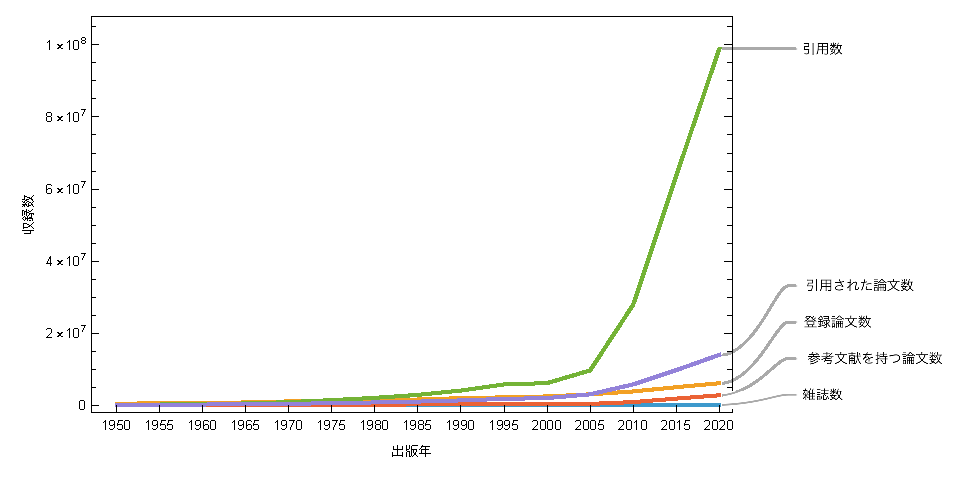
\includegraphics[width=75mm]{Main-manuscript_V4_gr2.eps}
  \caption{5年ごとの収録論文数}
  \label{fig:gr2}
\end{center}
\end{figure}


\subsection{Highly cited papers, journals publishing highly cited papers and highly-cited themes}
%本研究では、各累積世代において被引用数全体の1\%を構成する被引用数上位の論文群を「高被引用論文」と定義する。これらを掲載した雑誌を「高被引用論文掲載誌」、高被引用論文に付与されるMeSHディスクリプターを「高被引用テーマ」と定義する。さらに高被引用論文を引用する論文群を考え、これらの論文に付与されるMeSHディスクリプターを「高被引用論文引用テーマ」とする。
また、論文に付与されるMeSHディスクリプター一般を「研究テーマ」、論文が引用関係にある場合、引用される論文に付与されるMeSHディスクリプターを「被引用テーマ」、引用する論文に付与されるMeSHディスクリプターを「引用テーマ」とする。以上の定義をまとめたものを表\ref{tab:def}に示す。
また、本研究で示す論文の「年齢」は2020年時点の出版後からの年数である。

In this study, we define "highly cited papers" as the group of papers whose citation counts constitute the top1\% of all citations within each cumulative cohort. Journals that publish these papers are called "journals publishing highly cited papers", and the MeSH descriptors assigned to highly cited papers are termed "highly cited themes".

We also consider the set of papers that cite the highly cited papers; the MeSH descriptors attached to these citing papers are defined as "citing themes of highly cited papsers".

More generally, MeSH descriptors assigned to any paper are referred to as "research themes". When a citation relationship exists between two papers, the MeSH descriptors attached to the cited paper are called "cited themes", and those attached to the citing paper are called "citing themes".

A summary of these definitions is presented in Table\ref{tab:def}.

\begin{table}[h]
\begin{center}
\caption{本研究での用語定義} \label{tab:def}
{\small
\begin{tabular}{lp{32mm}}
  用語 & 定義 \\
  \hline 
  高被引用論文 & 被引用数全体の1\%を構成する被引用数上位論文 \\
  高被引用論文掲載誌 & 高被引用論文を出版した雑誌 \\
  高被引用テーマ & 高被引用論文に付与されるMeSHディスクリプター \\
  高被引用論文引用テーマ & 高被引用論文を引用する論文に付与されるMeSHディスクリプター \\
  研究テーマ & 論文に付与されるMeSHディスクリプター \\
  被引用テーマ & 論文に引用される論文に付与されるMeSHディスクリプター \\
  引用テーマ & 論文を引用する論文に付与されるMeSHディスクリプター \\
\end{tabular}
}
\end{center}
\end{table}


\subsection{Groups}
%のちに高被引用論文とその他の論文とを比較するため、各累積世代で高被引用論文を含め全4グループを構成する。論文を被引用数の大きい順に並べ、被引用数の累積和に基づいて総被引用数を100分した際の、累積被引用数の0-1\%区間に相当する論文群をG1すなわち高被引用論文、25-26\%区間にある論文群をG2、50-51\%区間にある論文群をG3、75-76\%区間にある論文群をG4とする。分位区間としないのはG2-G4における多様性を確保するためである。

Later, in order to compare highly cited papers with other papers, we form a total of four groups that include the highly cited papers. The highly cited papers constitute Group1 (G1); similarly, the set of papers whose citation counts fall in the top 25-26 percentile of the overall citation distribution is designated G2, those in the 50-51 percentile interval as G3, and those in the 75-76 percentile interval as G4.


\section{Highly cited papers}
\subsection{Occurrence of highly cited papers}
\begin{figure*}[t]
\centering

\begin{subfigure}{0.32\textwidth}
  \centering
  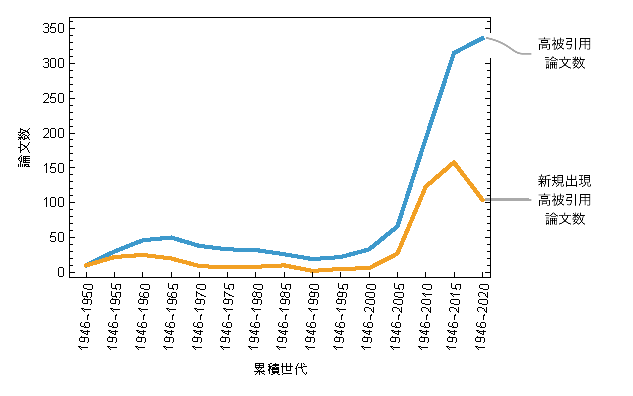
\includegraphics[width=\linewidth]{gr3.eps}
  \caption{高被引用論文および新規出現高被引用論文の出現数}
  \label{fig:gr3}
\end{subfigure}
\hfill
\begin{subfigure}{0.32\textwidth}
  \centering
  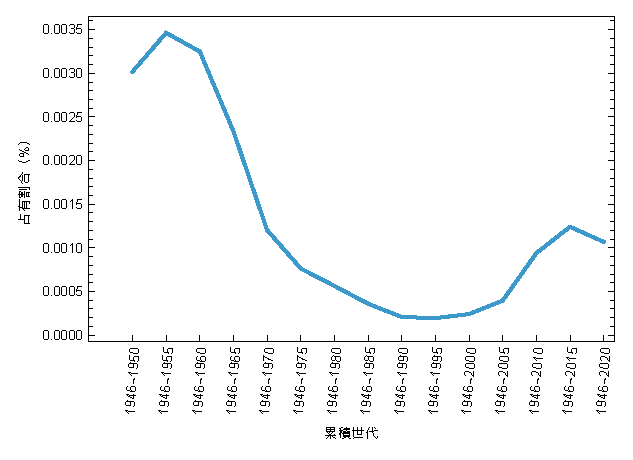
\includegraphics[width=\linewidth]{gr4.eps}
  \caption{高被引用論文の全論文に占める割合（\%）}
  \label{fig:gr4}
\end{subfigure}
\hfill
\begin{subfigure}{0.32\textwidth}
  \centering
  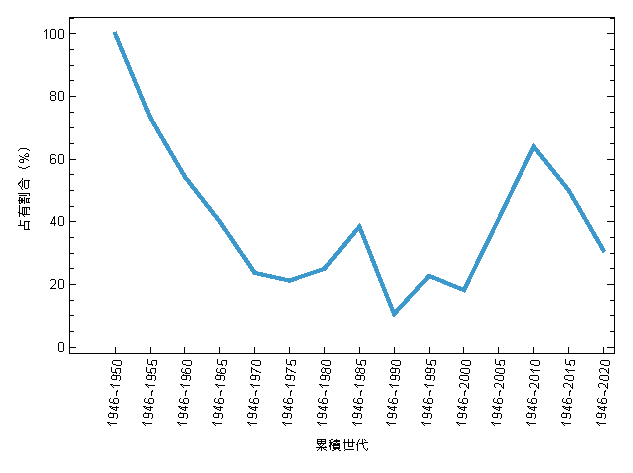
\includegraphics[width=\linewidth]{gr5.eps}
  \caption{新規出現高被引用論文の高被引用論文に占める割合（\%）}
  \label{fig:gr5}
\end{subfigure}

\caption{高被引用論文の統計}
\label{fig:array1all}
\end{figure*}

%全ての累積世代を通した、高被引用論文の総数（異なり）は536件であった。
累積世代ごとの出現数を図\ref{fig:gr3}に示す。高被引用論文数および新規出現高被引用論文数は1946-2010年の累積世代以降に急増しているが、これは近年の収録論文数の急増を受けたものであると考えられる。
高被引用論文の影響性を確認するため、高被引用論文の全論文に占める割合を図\ref{fig:gr4}に示す。 各累積世代の高被引用論文は出版数の割合としては0.0002-0.0035\%を占めているにすぎないが、これが被引用数の1\%を構成しており、被引用の集中の高さが見られる。値の変化に一定の傾向はなく緩やかな変動が見られる。
高被引用論文の累積世代ごとの入れ替わりを確認するため、新規高被引用論文の高被引用論文に占める割合を図\ref{fig:gr5}に示す。値の変化に一定の傾向は観察されず、10\%から70\%のメンバーの入れ替わりが見られる。

The number of occurrences of highly cited papers is shown in Figure\ref{fig:gr3}.
Both the total number of highly cited papers and the number of newly appearing highly cited papers increase sharply after the cumulative generation spanning 1946-2010, which is thought to reflect the recent rapid rise in the number of indexed papers.

To assess the impact of highly cited papers, the proportion of highly cited papers among all papers is shown in Figure\ref{fig:gr4}.
Highly cited papers constitute only 0.0002-0.0035\% of the total publications, yet they account for 1\% of citations, indicating a high concentration of citations. No consistent trend over time is observed, but a gentle fluctuation can be seen.

To examine the turnover of highly cited papers across cumulative generations, the proportion of newly highly cited papers within the set of highly cited papers is shown in Figure\ref{fig:gr5}. No consistent temporal trend is observed, and roughly a turnover of members ranging from 10-70\% is evident.


\subsection{Changes of highly cited papers}
%ここでは、高被引用論文の変遷をさらに詳しく見るために論文順位の変動を観察する。
Kendallの順位相関を用いた比較を年ごとに行えば、相関係数が高いほど順位変動が少ない、すなわち安定していると見做せる。
対象はすべての累積世代の高被引用論文とし、1947-2020年までの各年につき、前年と比較した際の相関係数を算出した。
図\ref{fig:gr101}に各年の相関係数を示す。
値は0.85-0.99の間を推移し、経過年による傾向は見られない。
さらに、累積的な被引用の効果がどのように現れるかを確認するため、出版後n年までの累積被引用数を用いた場合の相関係数も同図に示す。
これによれば、影響年を大きくするほど相関係数が小さくなる、すなわち順位が不安定化する傾向が見られ、被引用における累積的な影響は順位を変動させる要因となる可能性が高い。

Here, we observe the difference of paper rankings to further examine the evolution of highly cited papers in detail. 
By performing year-by-year comparisons using Kendall's rank correlation, a higher correlation coefficient implies less variation in rankings, i.e., greater stability. 
The subjects were the highly cited papers from all accumulated generations. For each year from 1947 to 2020, we calculated the correlation coefficient relative to the previous year. Figure \ref{fig:gr101} shows the correlation coefficients for each year. The values fluctuated between 0.85 and 0.99, with no discernible trend over the years. 

Furthermore, to examine how the cumulative effect of citations manifests, the figure also displays the correlation coefficients calculated using cumulative citations within $n$ years after publication. 
According to these results, as the citation window (impact years) increases, the correlation coefficient tends to decrease, indicating a tendency for rankings to become unstable. This suggests that the cumulative effect of citations is likely a factor driving fluctuations in paper rankings.

%次に、個別論文の代表としての最多被引用論文の変遷を確認する。各累積世代の最多被引用論文とその被引用数を表\ref{tab:mostcitedA}に示す。最多被引用論文は累積世代が進んでも引き続き引用され続ける傾向があり、数十年をかけてインパクトを上昇させている。このため最多被引用論文の交代は少ない。

Next, we examine the evolution of the most-cited paper as a representative of individual papers. Table \ref{tab:mostcitedA} presents the most-cited paper and its citation count for each cumulative generation. The most-cited papers tend to continue accumulating citations as cumulative generations progress, thereby increasing their impact over several decades. Consequently, the turnover of the most-cited paper is rare.

\begin{figure}[h]
\begin{center}
  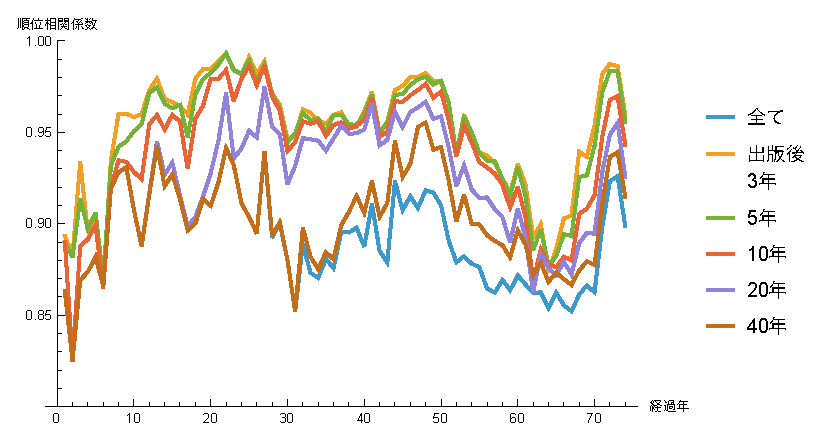
\includegraphics[width=76mm]{kendallall.eps}
  \caption{高被引用論文の順位相関係数 \newline すべての累積を用いた順相関係数と出版後n 年まで
の累積を用いた順位相関係数。}
  \label{fig:gr101}
\end{center}
\end{figure}

\begin{table*}[h]
\begin{center}
\caption{最多被引用論文} \label{tab:mostcitedA}
{\small
\[\begin{array}{cp{36mm}p{20mm}p{28mm}rr}
 {累積世代} & {\begin{tabular}{c}用論文タイトル\end{tabular}} & {\begin{tabular}{c}掲載誌タイトル\end{tabular}} & {被引用テーマ} & {被引用数} & {\begin{tabular}{c}当該累積世代\\の高被引用\\論文数\end{tabular}} \\ \hline
 {1946-1950} & {Qualitative analysis of proteins: a partition chromatographic method using paper} & {The Biochemical journal} & -
& 74 & 10 \\
 {1946-1955} & {上記と同じ} & {上記と同じ} & {上記と同じ} & 154 & 30 \\
 {1946-1960} & {Protein measurement with the Folin phenol reagent} & {The Journal of biological chemistry} & 
 {Molybdenum} / {Phenols} / {Plant Extracts} / {Proteins} / {Tungsten Compounds} 
 & 300 & 46 \\
 {1946-1965} & {上記と同じ} & {上記と同じ} & {上記と同じ} & 1190 & 50 \\
 {1946-1970} & {上記と同じ} & {上記と同じ} & {上記と同じ} & 3876 & 38 \\
 {1946-1975} & {上記と同じ} & {上記と同じ} & {上記と同じ} & 9632 & 33 \\
 {1946-1980} & {上記と同じ} & {上記と同じ} & {上記と同じ} & 17763 & 32 \\
 {1946-1985} & {上記と同じ} & {上記と同じ} & {上記と同じ} & 25451 & 26 \\
 {1946-1990} & {上記と同じ} & {上記と同じ} & {上記と同じ} & 32371 & 19 \\
 {1946-1995} & {上記と同じ} & {上記と同じ} & {上記と同じ} & 37576 & 22 \\
 {1946-2000} & {上記と同じ} & {上記と同じ} & {上記と同じ} & 40229 & 33 \\
 {1946-2005} & {上記と同じ} & {上記と同じ} & {上記と同じ} & 42101 & 66 \\
 {1946-2010} & {上記と同じ} & {上記と同じ} & {上記と同じ} & 44884 & 192 \\
 {1946-2015} & {Cleavage of structural proteins during the assembly of the head of bacteriophage T4} & {Nature} & 
 {Autoradiography} / {Carbon Isotopes} / {Coliphages} / {Electrophoresis, Disc} / {Genes} / {Genetics, Microbial} / {Kinetics} / {Viral Proteins} 
 & 49961 & 315 \\
 {1946-2020} & {上記と同じ} & {上記と同じ} & {上記と同じ} & 54249 & 336 \\
\end{array}\]
}
\end{center}
\end{table*}


\subsection{高被引用論文のオブソレッセンス}
ここでは、高被引用論文の影響が長期的にどのように変化するかを分析するため、オブソレッセンスに注目し、寿命構造を観察する。
まず、オブソレッセンス状態を判定するために、Sun\cite{SUn1}らの提案する Obsolescence vector を導入する。
Obsolescence vector はGini係数の派生であり$O(Gs,A^-)$で表されるが、本研究では$O(Gs,A^-,A^+)$を用いる。$Gs$は、値が小さいほど相対的に引用が早期に偏っていることを示し、$|A^-|$、$|A^+|$の値はそれぞれ被引用の減少および増加の変化の速さを示す（図\ref{fig:obsvec}）。

\begin{itemize}
\item FP; Flash in the pan：Sunらは Flash in the pan の基準として、$Gs=-0.600$、$A^- = -0.300$ を示している。本研究ではこの値を参照し、$Gs < -0.600$ かつ $A^- < -0.300$ の値を持つ論文を Flash in the pan とする。
\item SB; Sleeping beauty：Sunらは $A^+$ を用いた Sleeping beauty の基準を示していないが、本研究では Flash in the pan と対照的な条件として $Gs > 0.600$ かつ $A^+ > 0.300$ の値を持つ論文を Sleeping beauty とする。
\item Nm; 成熟論文：Flash in the pan にも Sleeping beauty にも含まれない標準的かつある程度引用を得た論文の条件として、$-0.600 \leq Gs \leq 0.600$ かつ $A^- < 0$ かつ $A^+ > 0$ かつ $|A^-| > |A^+|$ を設定し、これに当てはまる論文を成熟論文とする。
\item No; 成熟論文のうちオブソレッセンスが確認されるもの：成熟論文のうちオブソレッセンスの傾向が強いものとして $A^- < -0.1$ となる論文集合を設定する。
\item G; 成長論文：被引用が成長段階にある論文として、$-0.600 \leq Gs \leq 0.600$ かつ $A^- = 0$ を設定する。
\item O; その他：以上の条件に含まれないものとして特殊な被引用形状のものが考えられる。
\end{itemize}

\begin{figure}[h]
\begin{center}
  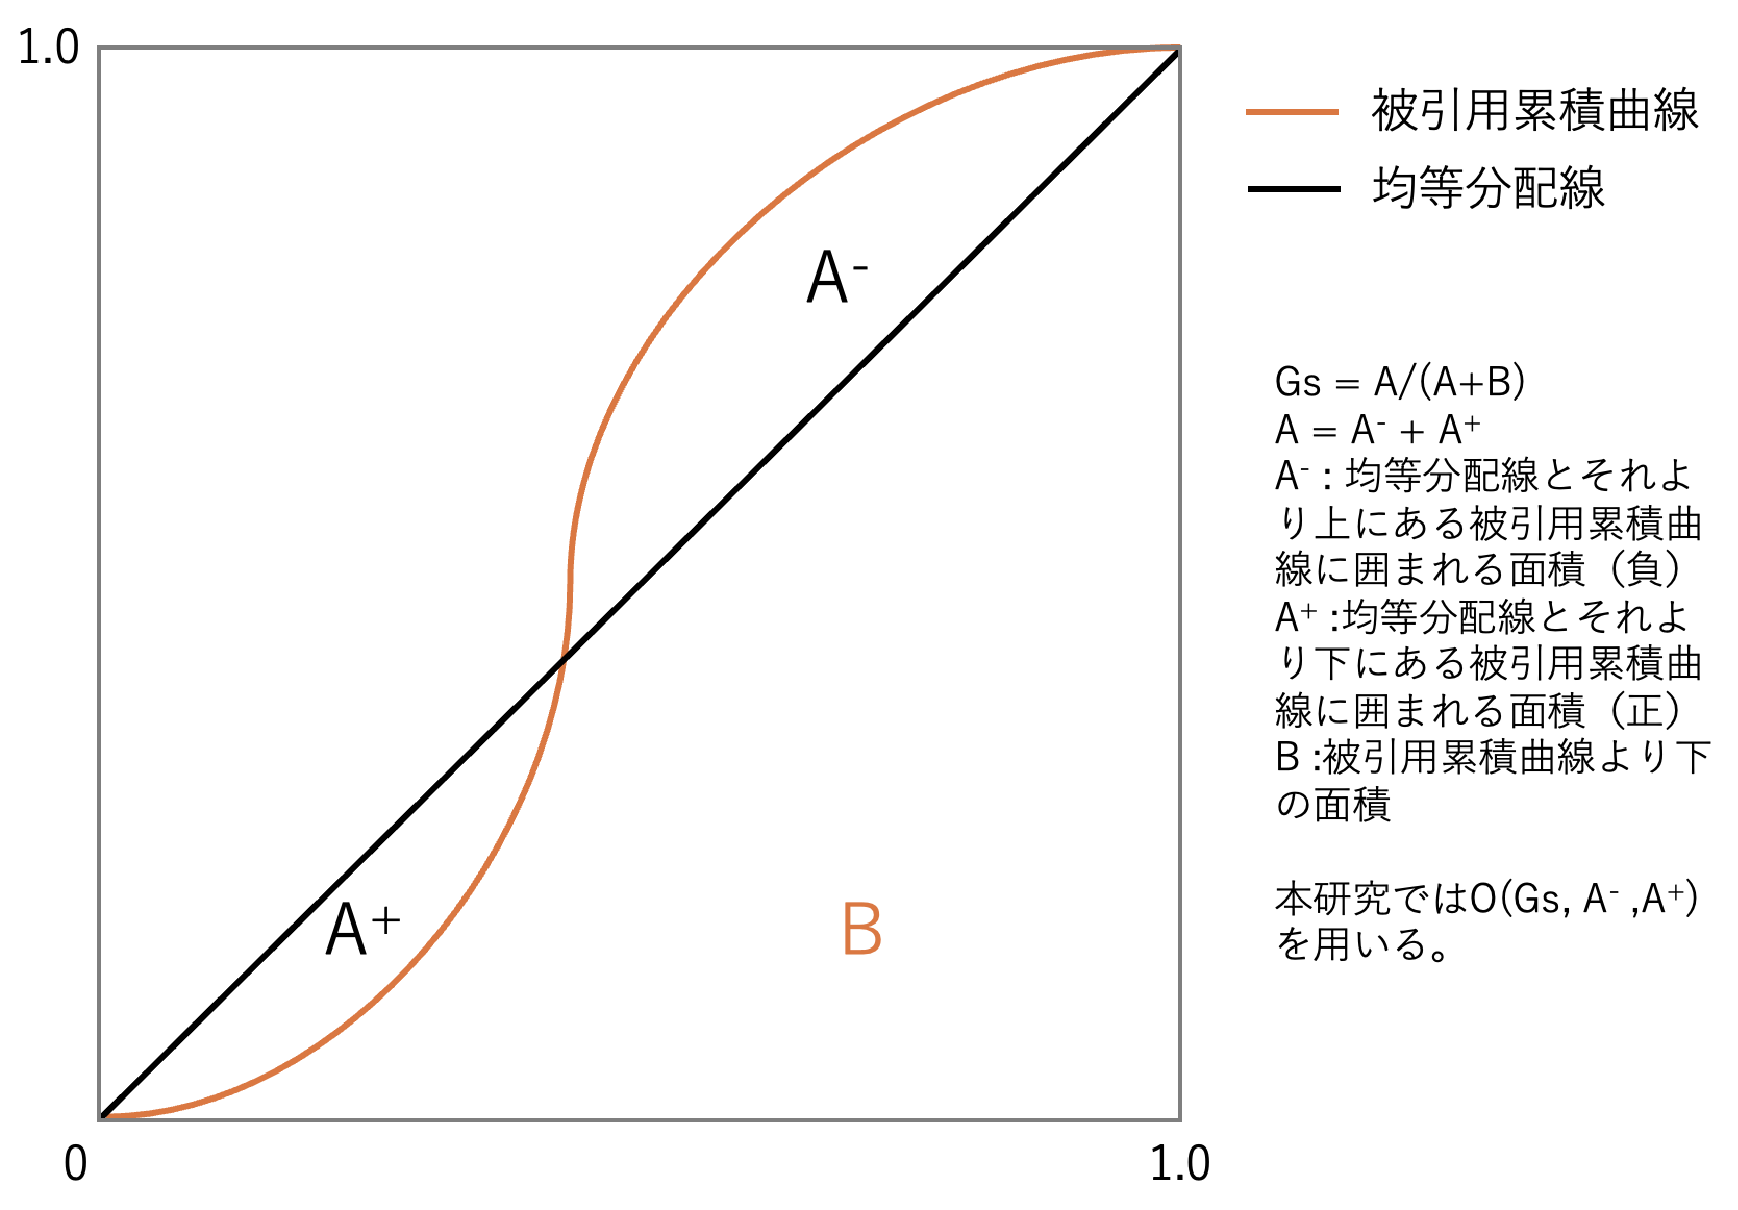
\includegraphics[width=76mm]{obsvec.eps}
  \caption{Obsolescence vector}
  \label{fig:obsvec}
\end{center}
\end{figure}

表\ref{tab:obsindex}に各クラスの指標値（中央値）を示す。高被引用論文ではクラスG（成長論文）が最も多く、次にクラスNm、クラスOと続き、クラスFPとクラスSBは同程度に出現している。なお、クラスFP（Flash in the pan）の年齢が高いのは、このクラスに分類されるには、早期の高い被引用だけでなくその後の十分な低い被引用期間も要することによる。
表\ref{tab:mcpobsindex}に最多被引用論文の指標値を示す。最多被引用論文の各指標値の範囲は広く、必ずしも特定のクラスから出現するわけではないことを示唆している。なお、うち2本はクラスOに分類されているが、被引用曲線を確認したところ明確な多峰性が見られ、リバイバル論文であることが明らかであった。

次に、これらの特性が高被引用論文に特有のものであるかを確認するため、表\ref{tab:g2obsindex}にG2論文の指標値を示す。
本指標値の算出には十分な被引用数が必要であるため、比較するグループはG2論文のみとする。
このG2論文はG1論文と同様にすべての累積世代に出現した論文群である。
これらの表によれば高被引用論文G1はG2に比べ、年齢は高く、$Gs$の値が小さいものは少なく、$Gs$の値が大きいものは多くなる傾向にある。このような構成の差異は、高被引用をなす要因が、単なる論文の年齢のみではないことを示唆している。
また、十分に成熟しオブソレッセンスの傾向がみられる群、すなわちクラスNoのピーク年（出版から被引用ピークまでの期間、中央値）を、G1とG2とで確認したところ、G1は9.5年、G2は5年であり、既存の報告（前述Paroloら）と比べるとG1では長くなる傾向を見せ、G2では整合的であった。

\begin{table*}
\begin{center}
\caption{高被引用論文（G1）のオブソレッセンスにかかる各指標値（中央値）} \label{tab:obsindex}
\begin{tabular}{lllllr}
クラス & $A^-$ & $A^+$ & Gs & 年齢 & メンバー数(\%)\\
\hline
FP & -0.346 & 0. & -0.691 & 70. & 29(5) \\
Nm & -0.116 & 0.005 & -0.323 & 44. & 150(28) \\
No & -0.192 & 0.004 & -0.374 & 49.5 & 114(21) \\
G & 0. & 0.179 & 0.358 & 15. & 195(36) \\
SB & 0. & 0.336 & 0.671 & 35. & 30(6) \\
O & 0. & 0.094 & 0.187 & 19. & 132(25) \\
\end{tabular}
\end{center}
\end{table*}

\begin{table*}
\begin{center}
\caption{最多引用論文のオブソレッセンスにかかる各指標値} \label{tab:mcpobsindex}
\begin{tabular}{llllll}
論文タイトル（一部）& クラス & $A^-$ & $A^+$ & Gs & 年齢 \\
\hline
Qualitative analysis of ... & FP & -0.332 & 0. & -0.664 & 77. \\
Protein measurement with ... & O & -0.011 & 0.066 & -0.110 & 70.  \\
Cleavage of structural proteins ... & O & -0.015 & 0.052 & 0.076 & 51.  \\
\end{tabular}
\end{center}
\end{table*}

\begin{table*}
\begin{center}
\caption{G2論文のオブソレッセンスにかかる各指標値（中央値）} \label{tab:g2obsindex}
\begin{tabular}{lllllr}
クラス & $A^-$ & $A^+$ & Gs & 年齢 & メンバー数(\%)\\
&  &  &  &  & ↑↓ :G1との比較\\
\hline
FP & -0.347 & 0. & -0.694 & 51. & 11254(13↑ ) \\
Nm & -0.119 & 0.002 & -0.231 & 32. & 36575(41↑ ) \\
No & -0.198 & 0.001 & -0.392 & 40. & 20634(23↑ ) \\
G & 0. & 0.123 & 0.274 & 15. & 14288(16↓ ) \\
SB & 0. & 0.324 & 0.648 & 42. & 301(0↓ ) \\
O & -0.001 & 0.051 & 0.086 & 20. & 26603(30↓ ) \\
\end{tabular}
\end{center}
\end{table*}


\section{高被引用論文掲載誌}
引用の構造は出版媒体（雑誌）という制度的単位とも深く関係している。
そこで本章では論文レベルの特性が雑誌という切り口ではどのように現れるかを見るため、高被引用論文を掲載する雑誌（高被引用論文掲載誌）に注目する。

\subsection{高被引用論文掲載誌の出現}
\begin{figure*}[t]
\centering

\begin{subfigure}{0.32\textwidth}
  \centering
  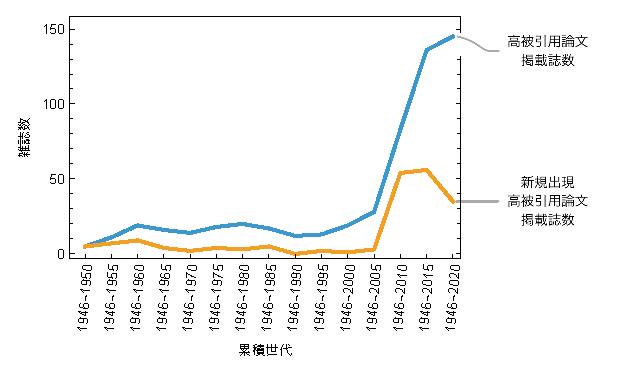
\includegraphics[width=\linewidth]{gr9.eps}
  \caption{高被引用論文掲載誌および新規出現高被引用論文掲載誌の出現数}
  \label{fig:gr9}
\end{subfigure}
\hfill
\begin{subfigure}{0.32\textwidth}
  \centering
  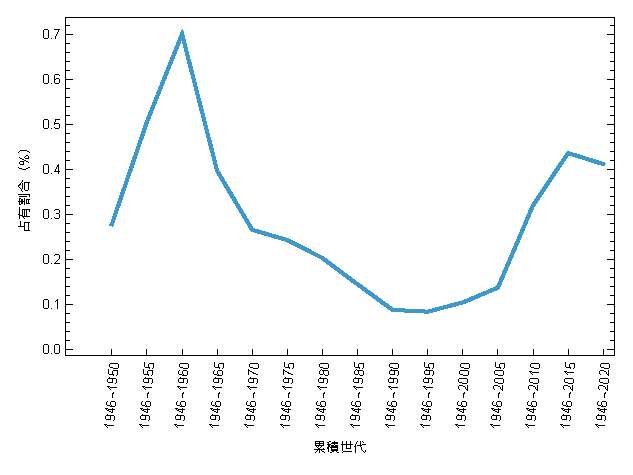
\includegraphics[width=\linewidth]{gr10.eps}
  \caption{高被引用論文掲載誌の全雑誌に占める割合（\%）}
  \label{fig:gr10}
\end{subfigure}
\hfill
\begin{subfigure}{0.32\textwidth}
  \centering
  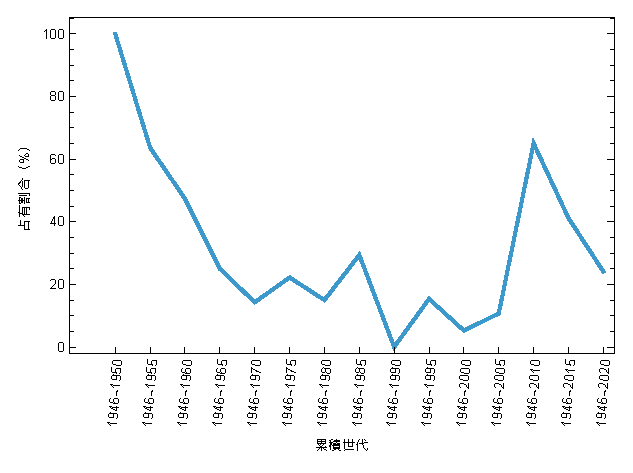
\includegraphics[width=\linewidth]{gr11.eps}
  \caption{新規出現高被引用論文掲載誌の高被引用論文掲載誌に占める割合（\%）}
  \label{fig:gr11}
\end{subfigure}

\caption{高被引用論文掲載誌の統計}
\label{fig:array2all}
\end{figure*}

高被引用論文掲載誌の出現数を図\ref{fig:gr9}に示す。高被引用論文掲載誌数および新規出現高被引用論文掲載誌は1946-2010年の累積世代以降に急増しており、前述した高被引用論文数の急増のタイミングと一致する。
おそらくこのタイミングで収録雑誌も増加したことが窺える。
高被引用論文掲載誌の影響性を確認するため、高被引用論文掲載誌の全雑誌に占める割合を図\ref{fig:gr10}に示す。値の変化に一定の傾向はなく緩やかな変動が観察される。高被引用論文掲載誌の入れ替わりを確認するため、新規出現高被引用論文掲載誌の高被引用論文掲載誌に占める割合を図\ref{fig:gr11}に示す。値の変化に一定の傾向は観察されず、かつ、激しい変動が観察される。


\subsection{高被引用論文掲載誌の変遷}
ここでは高被引用論文掲載誌の変化を高被引用でないグループのそれと比較する。
まず、G1-G4の代表として、当該グループ内での被引用数最上位の論文の掲載誌を表\ref{tab:G1topj}-\ref{tab:G4topj}に示す。
各誌のインパクトファクターとその発表年についてはJournal Citation Reports  (JCR）\cite{JCR1}から求めた。JCRではインパクトファクターの公開が1997からであるため、1946-2000年の累積世代以降についてのみ、累積世代の最終年のインパクトファクターを求めた。
ここから、高被引用論文を持つ雑誌は必ずしもインパクトファクターが高い雑誌ではないことが伺える。
一方、これらの表からは雑誌の構成においてはグループ間に特別な差異を認められない。
そこで、各グループでどの程度の雑誌の嗜好があるかを確認するため、全てのグループを統合した集合と各グループとの間でのKullback-Leibler divergence（KLD）を求めたものを図\ref{fig:gr12}に示す。同図からは、高被引用論文は他のグループに比べ雑誌の嗜好が強いことが窺え、この嗜好は年々強くなる傾向が見られる。

\begin{table*}[h]
\begin{center}
\caption{高被引用論文掲載誌のうち最大の高被引用論文数を持つもの} \label{tab:G1topj}
{\tiny
\[\begin{array}{ccccc}
 {累積世代} & 
\begin{array}{p{20mm}}
 {雑誌タイトル} \\
\end{array}
 & 
\begin{array}{p{14mm}}
 {当該誌の高被引用論文数} \\
\end{array}
 & 
\begin{array}{p{14mm}}
 {当該誌の高被引用論文が当該累積世代の高被引用論文全体に占める割合（\%）} \\
\end{array}
 & 
\begin{array}{c}
 {IF/発表年} \\
\end{array}
 \\
\hline
 {1946-1950} & 
\begin{array}{p{20mm}}
 {The Journal of clinical investigation} \\
 {The Biochemical journal} \\
\end{array}
 & 
\begin{array}{c}
 3 \\
 3 \\
\end{array}
 & 30 & 
\begin{array}{c}
 {12.015/2000}; {15.053/2005}; {14.152/2010}; {12.575/2015}; {14.808/2020} \\
 {4.28/2000}; {4.224/2005}; {5.016/2010}; {3.562/2015}; {3.857/2020} \\
\end{array}
 \\
 {1946-1955} & 
\begin{array}{p{20mm}}
 {上記と同じ} \\
\end{array}
 & 
\begin{array}{c}
 13 \\
\end{array}
 & 43 & 
\begin{array}{c}
 {上記と同じ} \\
\end{array}
 \\
 {1946-1960} & 
\begin{array}{p{20mm}}
 {上記と同じ} \\
\end{array}
 & 
\begin{array}{c}
 11 \\
\end{array}
 & 24 & 
\begin{array}{c}
 {上記と同じ} \\
\end{array}
 \\
 {1946-1965} & 
\begin{array}{p{20mm}}
 {上記と同じ} \\
\end{array}
 & 
\begin{array}{c}
 13 \\
\end{array}
 & 26 & 
\begin{array}{c}
 {上記と同じ} \\
\end{array}
 \\
 {1946-1970} & 
\begin{array}{p{20mm}}
 {上記と同じ} \\
\end{array}
 & 
\begin{array}{c}
 9 \\
\end{array}
 & 24 & 
\begin{array}{c}
 {上記と同じ} \\
\end{array}
 \\
 {1946-1975} & 
\begin{array}{p{20mm}}
 {The Journal of biological chemistry} \\
\end{array}
 & 
\begin{array}{c}
 7 \\
\end{array}
 & 21 & 
\begin{array}{c}
 {7.368/2000}; {5.854/2005}; {5.328/2010}; {4.258/2015}; {5.157/2020} \\
\end{array}
 \\
 {1946-1980} & 
\begin{array}{p{20mm}}
 {上記と同じ} \\
\end{array}
 & 
\begin{array}{c}
 7 \\
\end{array}
 & 22 & 
\begin{array}{c}
 {上記と同じ} \\
\end{array}
 \\
 {1946-1985} & 
\begin{array}{p{20mm}}
 {上記と同じ} \\
\end{array}
 & 
\begin{array}{c}
 5 \\
\end{array}
 & 19 & 
\begin{array}{c}
 {上記と同じ} \\
\end{array}
 \\
 {1946-1990} & 
\begin{array}{p{20mm}}
 {上記と同じ} \\
\end{array}
 & 
\begin{array}{c}
 4 \\
\end{array}
 & 21 & 
\begin{array}{c}
 {上記と同じ} \\
\end{array}
 \\
 {1946-1995} & 
\begin{array}{p{20mm}}
 {上記と同じ} \\
\end{array}
 & 
\begin{array}{c}
 4 \\
\end{array}
 & 18 & 
\begin{array}{c}
 {上記と同じ} \\
\end{array}
 \\
 {1946-2000} & 
\begin{array}{p{20mm}}
 {Journal of molecular biology} \\
 {Proceedings of the National Academy of Sciences of the United States of America} \\
\end{array}
 & 
\begin{array}{c}
 4 \\
 4 \\
\end{array}
 & 12 & 
\begin{array}{c}
 {5.388/2000}; {5.229/2005}; {4.008/2010}; {4.517/2015}; {5.469/2020} \\
 {10.789/2000}; {10.231/2005}; {9.771/2010}; {9.423/2015}; {11.205/2020} \\
\end{array}
 \\
 {1946-2005} & 
\begin{array}{p{20mm}}
 {Proceedings of the National Academy of Sciences of the United States of America} \\
\end{array}
 & 
\begin{array}{c}
 8 \\
\end{array}
 & 12 & 
\begin{array}{c}
 {10.789/2000}; {10.231/2005}; {9.771/2010}; {9.423/2015}; {11.205/2020} \\
\end{array}
 \\
 {1946-2010} & 
\begin{array}{p{20mm}}
 {Proceedings of the National Academy of Sciences of the United States of America} \\
 {Nature} \\
\end{array}
 & 
\begin{array}{c}
 14 \\
 14 \\
\end{array}
 & 7 & 
\begin{array}{c}
 {10.789/2000}; {10.231/2005}; {9.771/2010}; {9.423/2015}; {11.205/2020} \\
 {25.814/2000}; {29.273/2005}; {36.104/2010}; {38.138/2015}; {49.962/2020} \\
\end{array}
 \\
 {1946-2015} & 
\begin{array}{p{20mm}}
 {Nature} \\
\end{array}
 & 
\begin{array}{c}
 20 \\
\end{array}
 & 6 & 
\begin{array}{c}
 {25.814/2000}; {29.273/2005}; {36.104/2010}; {38.138/2015}; {49.962/2020} \\
\end{array}
 \\
 {1946-2020} & 
\begin{array}{p{20mm}}
 {Bioinformatics (Oxford, England)} \\
\end{array}
 & 
\begin{array}{c}
 17 \\
\end{array}
 & 5 & 
\begin{array}{c}
 {3.409/2000}; {6.019/2005}; {4.877/2010}; {5.766/2015}; {6.937/2020} \\
\end{array}
 \\
\end{array}\]
}
\end{center}
\end{table*}

\begin{table*}[h]
\begin{center}
\caption{G2論文掲載誌のうち最大のG2論文数を持つもの} \label{tab:G2topj}
{\tiny
\[\begin{array}{cp{20mm}ccc}
 {累積世代} & {雑誌タイトル} & {当該誌のG2論文数} & {\begin{array}{p{14mm}}当該誌のG2論文が当該累積世代のG2論文全体に占める割合（\%）\end{array}} & {IF / 発表年} \\
\hline
 {1946-1950} & {Journal of bacteriology} & 34 & 45 & {3.506/2000; 4.167/2005; 3.726/2010; 3.198/2015; 3.49/2020} \\
 {1946-1955} & {The Biochemical journal} & 20 & 7 & {4.28/2000; 4.224/2005; 5.016/2010; 3.562/2015; 3.857/2020} \\
 {1946-1960} & {上記と同じ} & 64 & 10 & {上記と同じ} \\
 {1946-1965} & {上記と同じ} & 62 & 7 & {上記と同じ} \\
 {1946-1970} & {The Journal of biological chemistry} & 90 & 6 & {7.368/2000; 5.854/2005; 5.328/2010; 4.258/2015; 5.157/2020} \\
 {1946-1975} & {The Journal of physiology} & 98 & 5 & {4.455/2000; 4.272/2005; 5.139/2010; 4.731/2015; 5.182/2020} \\
 {1946-1980} & {The Journal of biological chemistry} & 150 & 5 & {7.368/2000; 5.854/2005; 5.328/2010; 4.258/2015; 5.157/2020} \\
 {1946-1985} & {Proceedings of the National Academy of Sciences of the United States of America} & 214 & 6 & {10.789/2000; 10.231/2005; 9.771/2010; 9.423/2015; 11.205/2020} \\
 {1946-1990} & {上記と同じ} & 316 & 7 & {上記と同じ} \\
 {1946-1995} & {上記と同じ} & 410 & 7 & {上記と同じ} \\
 {1946-2000} & {上記と同じ} & 490 & 7 & {上記と同じ} \\
 {1946-2005} & {上記と同じ} & 715 & 7 & {上記と同じ} \\
 {1946-2010} & {上記と同じ} & 947 & 6 & {上記と同じ} \\
 {1946-2015} & {上記と同じ} & 882 & 5 & {上記と同じ} \\
 {1946-2020} & {Proceedings of the National Academy of Sciences of the United States of America} & 810 & 3 & {10.789/2000; 10.231/2005; 9.771/2010; 9.423/2015; 11.205/2020} \\
\end{array}\]
}
\end{center}
\end{table*}

\begin{table*}[h]
\begin{center}
\caption{G3論文掲載誌のうち最大のG3論文数を持つもの} \label{tab:G3topj}
{\tiny
\[\begin{array}{cp{20mm}ccc}
 {累積世代} & {雑誌タイトル} & {当該誌のG3論文数} & {\begin{array}{p{14mm}}当該誌のG3論文が当該累積世代のG3論文全体に占める割合（\%）\end{array}} & {IF / 発表年} \\
\hline
 {1946-1950} & {The Biochemical journal} & 41 & 24 & {4.28/2000; 4.224/2005; 5.016/2010; 3.562/2015; 3.857/2020} \\
 {1946-1955} & {The Journal of biological chemistry} & 21 & 4 & {7.368/2000; 5.854/2005; 5.328/2010; 4.258/2015; 5.157/2020} \\
 {1946-1960} & {Proceedings of the Society for Experimental Biology and Medicine. Society for Experimental Biology and Medicine
(New York, N.Y.)} & 71 & 5 & {3.415/2000; -/2005; -/2010; -/2015; -/2020} \\
 {1946-1965} & {The Journal of biological chemistry} & 72 & 3 & {7.368/2000; 5.854/2005; 5.328/2010; 4.258/2015; 5.157/2020} \\
 {1946-1970} & {上記と同じ} & 116 & 3 & {上記と同じ} \\
 {1946-1975} & {上記と同じ} & 205 & 4 & {上記と同じ} \\
 {1946-1980} & {上記と同じ} & 267 & 4 & {上記と同じ} \\
 {1946-1985} & {Proceedings of the National Academy of Sciences of the United States of America} & 388 & 4 & {10.789/2000; 10.231/2005; 9.771/2010; 9.423/2015; 11.205/2020} \\
 {1946-1990} & {The Journal of biological chemistry} & 440 & 4 & {7.368/2000; 5.854/2005; 5.328/2010; 4.258/2015; 5.157/2020} \\
 {1946-1995} & {上記と同じ} & 782 & 5 & {上記と同じ} \\
 {1946-2000} & {上記と同じ} & 897 & 5 & {上記と同じ} \\
 {1946-2005} & {上記と同じ} & 1419 & 5 & {上記と同じ} \\
 {1946-2010} & {上記と同じ} & 1681 & 4 & {上記と同じ} \\
 {1946-2015} & {上記と同じ} & 1976 & 4 & {上記と同じ} \\
 {1946-2020} & {上記と同じ} & 1678 & 2 & {上記と同じ} \\
\end{array}\]
}
\end{center}
\end{table*}

\begin{table*}[h]
\begin{center}
\caption{G4論文掲載誌のうち最大のG4論文数を持つもの} \label{tab:G4topj}
{\tiny
\[\begin{array}{cp{20mm}ccc}
 {累積世代} & {雑誌タイトル} & {当該誌のG4論文数} & {\begin{array}{p{14mm}}当該誌のG4論文が当該累積世代のG4論文全体に占める割合（\%）\end{array}} & {IF / 発表年} \\
\hline
 {1946-1950} & {Annals of surgery} & 34 & 10 & {5.987/2000; 6.328/2005; 7.474/2010; 8.569/2015; 12.969/2020} \\
 {1946-1955} & {上記と同じ} & 105 & 6 & {上記と同じ} \\
 {1946-1960} & {The Biochemical journal} & 240 & 10 & {4.28/2000; 4.224/2005; 5.016/2010; 3.562/2015; 3.857/2020} \\
 {1946-1965} & {Nature} & 121 & 3 & {25.814/2000; 29.273/2005; 36.104/2010; 38.138/2015; 49.962/2020} \\
 {1946-1970} & {British medical journal} & 185 & 2 & {5.331/2000; 9.052/2005; 13.471/2010; -/2015 -/2020} \\
 {1946-1975} & {Biochimica et biophysica acta} & 290 & 3 & {-/2000; -/2005; -/2010; -/2015; -/2020} \\
 {1946-1980} & {上記と同じ} & 489 & 3 & {上記と同じ} \\
 {1946-1985} & {The Journal of biological chemistry} & 627 & 3 & {7.368/2000; 5.854/2005; 5.328/2010; 4.258/2015; 5.157/2020} \\
 {1946-1990} & {Biochimica et biophysica acta} & 842 & 3 & {-/2000; -/2005; -/2010; -/2015; -/2020} \\
 {1946-1995} & {The Journal of biological chemistry} & 1142 & 3 & {7.368/2000; 5.854/2005; 5.328/2010; 4.258/2015; 5.157/2020} \\
 {1946-2000} & {上記と同じ} & 1770 & 4 & {上記と同じ} \\
 {1946-2005} & {上記と同じ} & 1375 & 2 & {上記と同じ} \\
 {1946-2010} & {上記と同じ} & 2093 & 2 & {上記と同じ} \\
 {1946-2015} & {PloS one} & 3117 & 2 & {-/2000; -/2005; 4.411/2010; 3.057/2015; 3.24/2020} \\
 {1946-2020} & {上記と同じ} & 3560 & 2 & {上記と同じ} \\
\end{array}\]
}
\end{center}
\end{table*}

\begin{figure}[h]
\begin{center}
  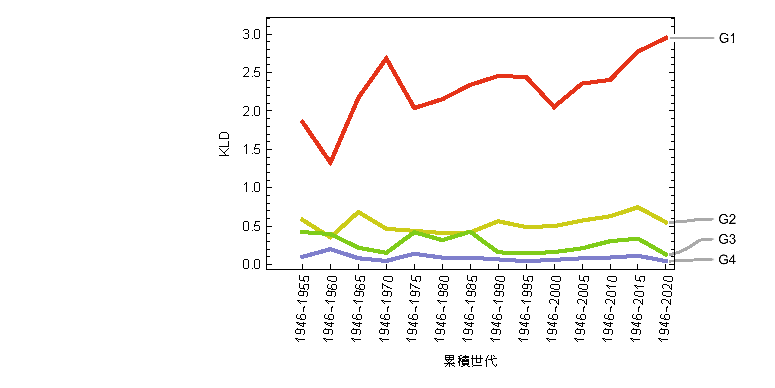
\includegraphics[width=75mm]{Main-manuscript_V4_gr12.eps}
  \caption{各グループの雑誌の構成に関するKLD}
  \label{fig:gr12}
\end{center}
\end{figure}


\section{高被引用テーマ}
本章ではさらに視点を変え、研究内容に関する構造的な差を明らかにするため論文のテーマに着目する。

\begin{figure*}[t]
\centering

\begin{subfigure}{0.32\textwidth}
  \centering
  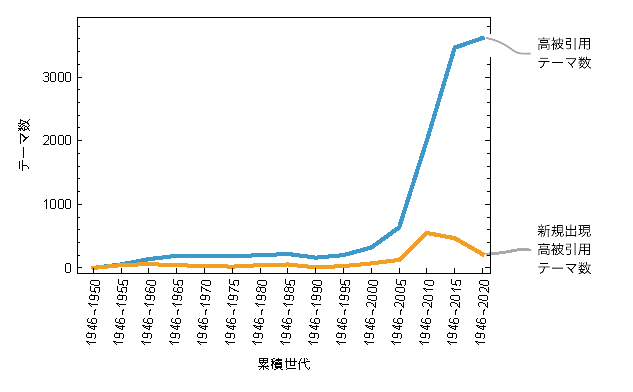
\includegraphics[width=\linewidth]{gr13.eps}
  \caption{高被引用テーマおよび新規出現高被引用テーマの出現数}
  \label{fig:gr13}
\end{subfigure}
\hfill
\begin{subfigure}{0.32\textwidth}
  \centering
  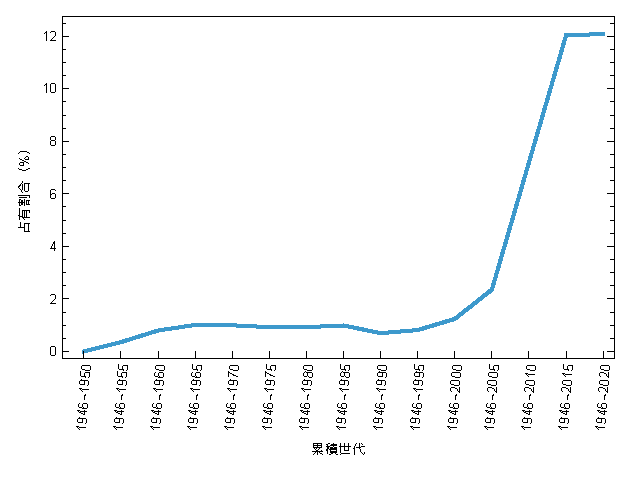
\includegraphics[width=\linewidth]{gradd1.eps}
  \caption{高被引用テーマの全出現テーマに占める割合（\%）}
  \label{fig:gradd1}
\end{subfigure}
\hfill
\begin{subfigure}{0.32\textwidth}
  \centering
  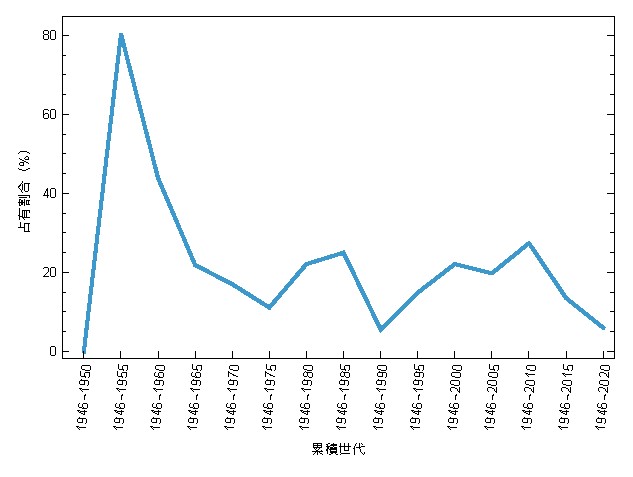
\includegraphics[width=\linewidth]{gr14.eps}
  \caption{新規出現高被引用テーマの高被引用テーマ全体に占める割合（\%）}
  \label{fig:gr14}
\end{subfigure}

\caption{高被引用論文掲載誌の統計}
\label{fig:array2all}
\end{figure*}

\subsection{高被引用テーマの出現}
高被引用テーマのユニーク出現数を図\ref{fig:gr13}に示す。2023年MeSHディスクリプターの総数はおよそ30000であるが、各累積世代における高被引用テーマの出現数は最大でも3000を超える程度であり高被引用テーマには集中が見られる。
高被引用テーマの全出現テーマに占める割合を図\ref{fig:gradd1}に示す。ここからは近年ほどそのテーマが多様化していることが窺える。
高被引用テーマの入れ替わりを確認するため、新規出現高被引用テーマの高被引用テーマ全体に占める割合を図\ref{fig:gr14}に示す。値の変化に一定の傾向は観察されず、初期の累積世代を除けば、数\%から30\%の範囲での入れ替わりが観察される。なお、1946-1955年の累積世代に高い値が見られる理由は、前累積世代ではMeSHディスクリプターの付与がほとんどなかったためである。


\subsection{高被引用テーマの変遷}
ここでは、高被引用テーマのさまざまな変化を、他のグループのそれと比較する。
各累積世代ごと、各グループごとの最頻出被引用テーマと引用テーマを表\ref{tab:topmesh}に示す。これらのうちG1の被引用テーマ（高被引用テーマ）にのみにバラエティが確認される。
次に、各累積世代の被引用テーマと引用テーマの多様性を見るために各グループのエントロピーの変化を観察した。被引用テーマ、引用テーマ、被引用テーマと引用テーマ対の出現数のエントロピーを、それぞれ図\ref{fig:arr2}に示す。計数の方法は、被引用テーマと引用テーマについては、それぞれ論文ごとの分数カウントを採用する。被引用テーマ対引用テーマのペアについては、ひとつの参照ごとに被引用テーマと引用テーマの2部グラフを構成し、エッジの重みの合計が1となる分数カウントを採用する。図\ref{fig:arr2}からは高被引用論文のみ、いずれのエントロピーも低く、その他のグループ間ではそれほど差がないことが窺える。なお、1946-1950年の累積世代に関してはMeSHディスクリプターの付与数が十分でなかったため除外している。
また、研究者の引用行動は必ずしも当該論文と同じテーマを引用するものではない。この転換の程度を見るために、グループごとに被引用テーマと引用テーマのコサイン距離を観察した。この結果を図\ref{fig:meshpivot}に示す。ここでも高被引用論文のみが累積世代の中期から後期にかけ他とは異なる様相を示した。また、高被引用論文は1946-2010年の累積世代以降、転換の程度は減少傾向にあり、他のグループとの差はなくなりつつあるように推察される。

\begin{table*}[h]
\begin{center}
\caption{累積世代ごと論文グループごとの最頻出テーマ} \label{tab:topmesh}
{\tiny
\[\begin{array}{c|cccc}
\begin{array}{c}
 { } \\
\hline
 {1946-1955} \\
 {1946-1960} \\
 {1946-1965} \\
 {1946-1970} \\
 {1946-1975} \\
 {1946-1980} \\
 {1946-1985} \\
 {1946-1990} \\
 {1946-1995} \\
 {1946-2000} \\
 {1946-2005} \\
 {1946-2010} \\
 {1946-2015} \\
 {1946-2020} \\
\end{array}
 & 
\begin{array}{cc}
 {G1引用テーマ} & {被引用テーマ} \\
\hline
 {Humans} & {Insulin} \\
 {Humans} & {Blood Proteins} \\
 {Animals} & {Microscopy, Electron} \\
 {Animals} & {Microscopy, Electron} \\
 {Animals} & {Microscopy, Electron} \\
 {Animals} & {Proteins} \\
 {Animals} & {Proteins} \\
 {Animals} & {Proteins} \\
 {Animals} & {Base Sequence} \\
 {Animals} & {Base Sequence} \\
 {Animals} & {Base Sequence} \\
 {Animals} & {Humans} \\
 {Humans} & {Humans} \\
 {Humans} & {Humans} \\
\end{array}
 & 
\begin{array}{cc}
 {G2引用テーマ} & {被引用テーマ} \\
\hline
 {Humans} & {Humans} \\
 {Humans} & {Humans} \\
 {Humans} & {Humans} \\
 {Humans} & {Humans} \\
 {Humans} & {Humans} \\
 {Humans} & {Humans} \\
 {Animals} & {Humans} \\
 {Animals} & {Animals} \\
 {Animals} & {Humans} \\
 {Animals} & {Animals} \\
 {Humans} & {Animals} \\
 {Humans} & {Humans} \\
 {Humans} & {Humans} \\
 {Humans} & {Humans} \\
\end{array}
 & 
\begin{array}{cc}
 {G3引用テーマ} & {被引用テーマ} \\
\hline
 {Humans} & {Humans} \\
 {Humans} & {Humans} \\
 {Humans} & {Humans} \\
 {Humans} & {Humans} \\
 {Humans} & {Humans} \\
 {Humans} & {Humans} \\
 {Humans} & {Animals} \\
 {Humans} & {Humans} \\
 {Humans} & {Humans} \\
 {Humans} & {Humans} \\
 {Humans} & {Humans} \\
 {Humans} & {Humans} \\
 {Humans} & {Humans} \\
 {Humans} & {Humans} \\
\end{array}
 & 
\begin{array}{cc}
 {G4引用テーマ} & {被引用テーマ} \\
\hline
 {Humans} & {Humans} \\
 {Humans} & {Humans} \\
 {Humans} & {Humans} \\
 {Humans} & {Humans} \\
 {Humans} & {Animals} \\
 {Humans} & {Humans} \\
 {Humans} & {Humans} \\
 {Humans} & {Humans} \\
 {Humans} & {Humans} \\
 {Humans} & {Humans} \\
 {Humans} & {Humans} \\
 {Humans} & {Humans} \\
 {Humans} & {Humans} \\
 {Humans} & {Humans} \\
\end{array}
 \\
\end{array}\]
}
\end{center}
\end{table*}

さらに、各累積世代間に対して被引用テーマの転換の程度を確認するために、各グループの累積世代間の被引用テーマのコサイン距離を観察する。各テーマのカウントには分数カウントを採用した。
この結果を図\ref{fig:gr15}に示す。G2だけが安定的な推移を示しているが、その他のグループは激しい値の変動が見られ、特段の傾向は読み取れない。

\begin{figure*}[h]
\begin{center}
  {\small
  \begin{tabular}{ccc}
  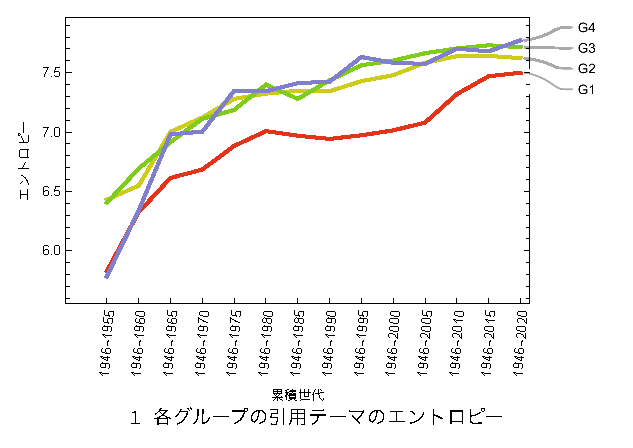
\includegraphics[width=55mm]{entropymesh-1.eps} & 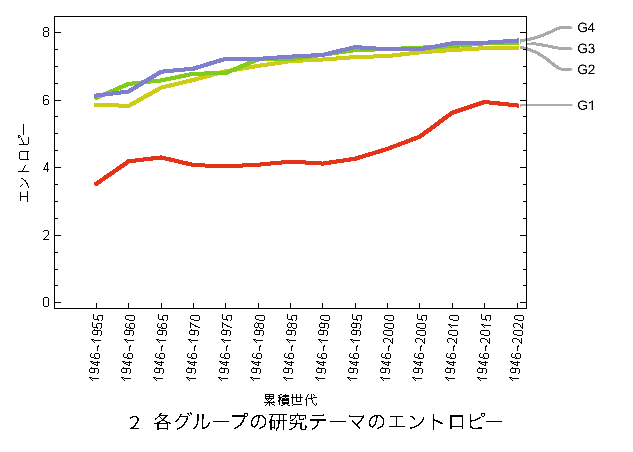
\includegraphics[width=55mm]{entropymesh-2.eps} & 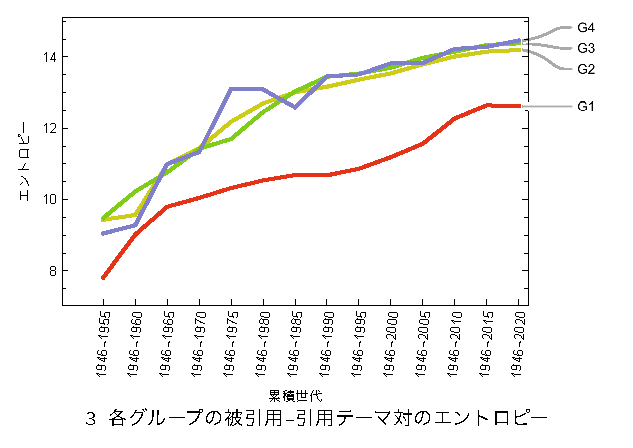
\includegraphics[width=55mm]{entropymesh-3.eps} \\
  \end{tabular}
  }
  \caption{累積世代、論文グループごとの研究テーマの出現に関するエントロピー}
  \label{fig:arr2}
\end{center}
\end{figure*}

\begin{figure}[h]
\begin{center}
  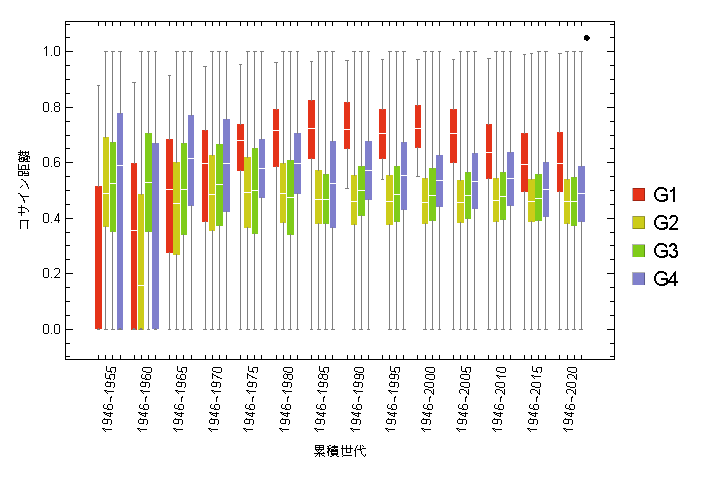
\includegraphics[width=76mm]{meshpivotatGen.eps}
  \caption{累積世代、論文グループごとの研究テーマに対する引用テーマの転換の程度}
  \label{fig:meshpivot}
\end{center}
\end{figure}

\begin{figure}[h]
\begin{center}
  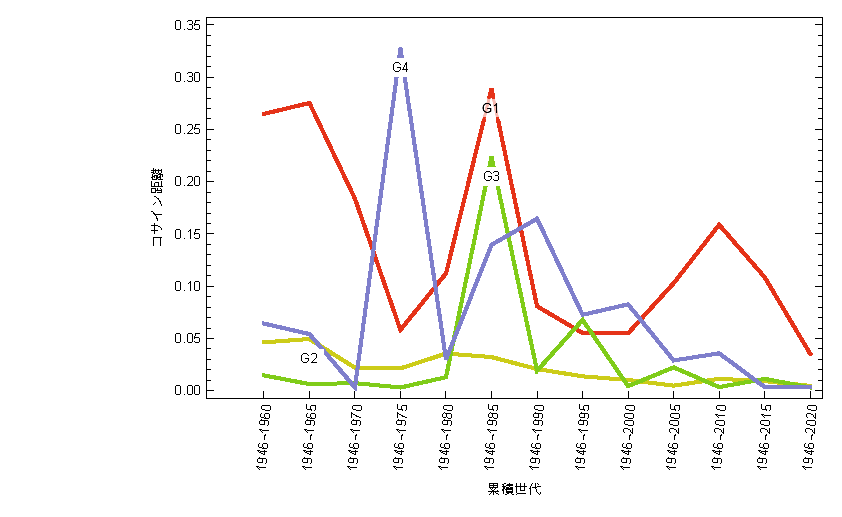
\includegraphics[width=75mm]{Main-manuscript_V4_gr15.eps}
  \caption{論文グループごとの累積世代間の研究テーマの転換の程度}
  \label{fig:gr15}
\end{center}
\end{figure}

以上より、高被引用論文には次の特徴があると考えられる：(1)高被引用論文は異なるテーマから引用されやすい。このことは表\ref{tab:topmesh}の最頻出テーマから予想され、図\ref{fig:meshpivot}に示す転換の程度もこれを裏付けている。
(2)高被引用論文は研究テーマが集中的であり、それを引用する論文の研究テーマもまた集中的である。このことは図\ref{fig:arr2}から示唆される。
(3)高被引用論文のテーマの多様性は、共時的には低いが通時的にはそうとは言えない。このことは、図\ref{fig:arr2}では他のグループに比べ低いエントロピーが観察される一方、図\ref{fig:gr15}では他のグループと比較して明確な差が見えないことによる。


\section{まとめ}
高被引用論文のオブソレッセンス：
高被引用論文はその被引用の累積的な効果により長期にわたり上位の順位を維持するものの、最終的には減衰が確認され、新しい累積世代の論文にその座を明け渡す現象を確認できた。この交代までの期間は非常に長く最長で50年以上であった。うち、オブソレッセンスが確認された論文集合では、既存の報告と比べ、出版から被引用数ピークまでの期間が長くなる傾向があった。

高被引用論文掲載誌の特徴：
高被引用論文が必ずしもトップクラスの高インパクトファクター誌に掲載されるわけではないことが明らかになった。つまり、実際にはよりインパクトファクターの高い雑誌が多く収録されているにもかかわらず、高被引用論文掲載誌においては、必ずしもそのような雑誌で占められているわけではない。
高被引用論文の雑誌への嗜好については、特定の雑誌へのそれは確認できなかったが、KLDによる分析から他のグループに比べより集中的であり、この傾向は年々強くなることが明らかになった。

高被引用テーマと高被引用論文引用テーマ：
高被引用論文は、研究テーマが集中的であり、異なるテーマの論文から引用されやすく、引用を行う側の論文の研究テーマもまた集中的であることが明らかになった。
高被引用論文は、被引用テーマおよび引用テーマそれぞれを個別に見た場合の多様性は低いが、被引用テーマ対引用テーマの転換という観点では転換の程度が高くなる。もしこれがオブソレッセンスに影響しているのだとすれば、様々な研究領域から興味を持たれるようなテーマの論文は長く引用され続けるのかもしれない。
この特徴がそのまま雑誌レベルに現れるとするならば、基礎分野あるいは学祭的な雑誌は各論文が比較的長く引用され続け、長期的には大きな影響を持つと考えられ、インパクトファクターのような短期的指標では測れない影響を持っている可能性が高い。

長期的な傾向：
本研究ではさまざまな指標を用いたが、長期的になんらかの傾向が見られたものは少なく、
引用テーマ/被引用テーマ/引用テーマ-被引用テーマ対のエントロピーに経過年による上昇傾向が見られ、高被引用論文の雑誌への嗜好にも経過年による上昇が見られた。

累積的な被引用データの影響：
累積的な集計の影響期間を変動させた順位相関の分析の結果、累積的な被引用を用いることにより順位の変動が大きくなった。すなわち累積的な被引用データを用いることは、順序尺度の評価においてダイナミクスを上昇させることにつながる。

最多被引用論文はどのような論文か？：
最後に、本研究で最多被引用論文となった3本の論文を俯瞰する。
\begin{itemize}
\item "Qualitative analysis of proteins: a partition chromatographic method using paper" は、実験手法に関する論文であり、ここで紹介される「ペーパークロマトグラフィ」は、この論文の著者らによって開発されたことで有名である。
\item "Protein measurement with the Folin phenol regent" は、実験手法に関する論文であり、著者（開発者）の名前にちなみ、「ローリー法」としてよく知られている。
\item "Cleavage of structural protein during the assembly of the head of bacteriophage T4" は、実験手法を紹介した論文であり、現在の「SDS-PAGE」法の原型となったことでよく知られている。
\end{itemize}
なお、2、3番目の論文は、Natureの記事 "The top 100 papers" \cite{Nor1}においても紹介（添付データとして）されている。


\section{本研究の限界と今後の課題}
本研究はPubMedという医学生物学分野に限られた範囲のデータにおける分析であり、他の分野、あるいはより広範な分野を対象とした場合に同様の結果と考察を得られるかは分からない。

一つの検証として、前述の最多被引用論文2本につき、本研究による被引用数と自然科学領域全体を対象とした"The top 100 papers"によるそれを比較（本研究の1946-2015累積世代とWeb of Scienceの2014年データ）すると、
"Protein measurement with the Folin phenol regent"では、前者で49164件および後者で305148件、
"Cleavage of structural protein during the assembly of the head of bacteriophage T4"では、前者で49916件および後者で213005件
であり、およそ4倍から6倍の差があり、同様の解釈はできない。
一方、双方に出現する論文タイトルを比較したところ、一致するタイトルも多数存在した。

雑誌レベルの観点では、"The top 100 papers"においても必ずしも高インパクトファクター誌が現れるとは限らないことが示されており、この点においては学際的領域においても医学生物学分野と同様の性質があると考えられる。

一方、研究テーマの分析に関して、本手法をより広範な分野に適応できるかという観点では、MeSHディスクリプターほどに整理された統制語を他のデータベースで利用することは難しく、本研究と同等の精度の分析は難しい。

以上を勘案した今後の現実的な課題としては、(1)PMCと同程度に整理されたコーパスを持つ異なる分野においての比較、(2)学際的な領域においても同程度の精度で分析をおこなうための、キーワードや学術領域ラベルの整理、が考えられる。


\section{データ利用可能性宣言}
本研究で利用したデータは、FTP版PubMed annual baseline（2023年）であり、同サービスはすでに提供されていない。
同様のデータが、現在では当該データを含むアップデートされたデータとしてS3サービスにより、 \\ https://pmc.ncbi.nlm.nih.gov/tools/pmcaws/ \\ から公開されている。
本研究で利用したプログラムソースコードは、 GitHub \\ https://github.com/kouamano/pubmed-analysis \\ より公開されている。


\balance
\bibliographystyle{ujsik}
\bibliography{ama.utf8}

\end{document}
